% !TEX encoding = UTF-8 Unicode
%!TEX root = thesis.tex

\newpage
\section{Background}

Prior to addressing the actual approach and implementation some concepts and terms have to be introduced. Firstly, the term \textit{security concept}, as it is used throughout the thesis, is being described. A definition of \textit{granularity levels} and system abstraction follows. Lastly, a section covers \textit{model transformations} and \textit{aggregation rules} on security attributes.

\subsection{Security}

Morrie Gasser \cite{Gasser} published a book in 1988 providing solutions for computer scpecialists interested in computer security. The term \textit{Computer Security} usually dealt with three aspects:

\begin{itemize}
\item Prevention of theft or damage to the hardware 
\item Prevention of theft or damage to the information
\item Prevention of service disruption
\end{itemize}

With the invention of the Internet the (personal) computers got interconnected and the sharing of data became prevalent and thus data security.

Nowadays security is seen as a process. No combination of products are guaranteed to make a system secure since they are only as secure as the people configuring them \cite{vacca2012computer}. \label{sec:security}

In general when talking about computer security three aspects are addressed, \textit{Confidentiality}, \textit{Integrity} and \textit{Availability} \cite{Pfleeger:2006:SC:1177321}. Each of them will no be defined:

\begin{itemize}
\item[] \textbf{Confidentiality} Assets can only be accessed by authorized parties
\item[] \textbf{Integrity} Assets can only be modified by authorized parties
\item[] \textbf{Availability} Assets are available to authorized parties when needed
\end{itemize} 

The challenge is seen in finding the right balance between the three \textit{Security Goals}. This situation is aggravated by the fact that the goals can overlap, be independent or even mutually exclusive. Charles P. Pfleeger \cite{Pfleeger:2006:SC:1177321} for example, addresses this problem by stating that a strong protection of confidentiality might restrict availability in a system.   

Information systems consist of hardware, software and data and it is of high importance for the respective stakeholder to secure the object of interest. When speaking about securing systems or components we look at two different terminologies, \textit{Vulnerabilities} and \textit{Threats}. A \textit{vulnerability} is a system weakness, be it in implementation or design, that can be potentially exploited by an adversary. Without the intent of exploiting it the vulnerability has no further effect on the system.

A \textit{threat} however is a set of circumstances that has the theoretical potential to cause harm by exploiting a specific vulnerability \cite{vacca2012computer}. An example to demonstrate the differences follows:

\begin{enumerate}[label=\textbf{Def.\arabic*}]
\item \textbf{Vulnerability}: Sending sensitive data over an unsecured channel \label{item:vuln}
\item \textbf{Threat}: Exploiting the unsecured channel by eavesdropping and gathering the sensitive data 
\end{enumerate}

As mentioned before a system weakness does not necessarily mean loss of data or any other system breach. Only when coupled with a set of circumstances and the intent of exploitation it turns into a threat. Figure \ref{fig:threats} illustrates the four acts that cause security harm as mentioned by Pfleeger \cite{Pfleeger:2006:SC:1177321}. 

\begin{figure}[H]
\centering
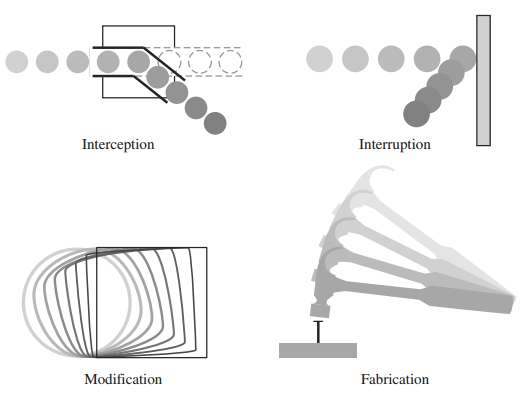
\includegraphics[width=0.85\textwidth]{pictures/threats.png}
\caption{Four acts that cause security harm}
\label{fig:threats}
\end{figure}

Confidentiality, integrity and availability, or the C-I-A triad like it is also being called, can be viewed from a perspective of the causes of harm. Confidentiality can suffer if some unauthorized party intercepts the data, availability can be lost if a flow of data is being interrupted and lastly integrity can be broken if the data is being modified or false data is being fabricated by an adversary.

To prevent the vulnerabilities from being exploited and the threats from potentially causing harm one can use \textit{Controls} or \textit{Countermeasures} to secure parts of a system. An example would be the use of encryption to prevent sensitive data from being eavesdropped on as mentioned in \ref{item:vuln}. 

To put everything into perspective the term \textit{Security Architecture} will be introduced.

\subsubsection{Security Architecture}

Gacek et al. discussed the definition of a \textit{Software System Architecture} (SSA) which will be used and adapted in the security context. According to the authors a \textit{Software System Architecture} is:

\begin{itemize}
\item A collection of software and system components, connections and constraints
\item A collection of system stakeholders' need statements
\item A rationale which demonstrates that the elements which define a system satisfy the the stakeholders' needs, if implemented correctly
\end{itemize}

Here, a \textit{Security Architecture} (SA) would be an adapted definition where, if implemented correctly, the stakerholders' \textit{security} needs will be satisfied. Naturally, the connections as well as the respective components might differ from the Software System Architecture as they might have to be enhanced or altered to satisfy the security needs. 

The stakeholders themselves however, are very similar. Gacek et al. differentiate between five parties, the \textit{Customer}, the \textit{User}, the \textit{Architect and System Engineer}, the \textit{Developer} and the \textit{Maintainer}. 

The International Standard ISO 27001 provides a model for establishing, impelementing, operating, monitoring, reviewing, maintaining and improving an organization's Information Security Management System \cite{iso27001}, i.e. a system that is responsible for establishing and maintaining organization's security needs and guidelines. When comparing these rather short definitions one can already see an overlap when looking at potential stakeholders. An overview on the SSA stakeholders follows:

\begin{tabular}{|c|c|}
\hline
Stakeholder & SSA Concern \\
\hline
Customer & \makecell{Schedule and budget estimation \\ Feasibility and risk assessment \\ Requirements traceability \\ Progress tracking} \\
\hline
User & \makecell{Consistency with requirements and usage scenarios \\ Future requirement growth accommodation \\ Performance, reliability, interoperability} \\
\hline
\makecell{Architect and \\ System Engineer} & \makecell{Requirements traceability \\ Support of tradeoff analyses \\ Completeness, consistency of architecture} \\
\hline
Developer & \makecell{Sufficient detail for design \\ Reference for selecting/assembling components \\ Maintain interoperability with existing systems} \\
\hline
Maintainer & \makecell{Guidance on software modification \\ Guidance on architecture evolution \\ Maintain interoperability with existing systems} \\
\hline
\end{tabular}      
\vspace{3mm}

When looking into the International Standard, one can see that similar concerns can be also found in the adaptation of the \glqq Plan-Do-Check-Act\grqq \ model for the establishment of an ISMS process. In the case of ISMS similar aspects can be found in the four different phases as seen in Figure \ref{fig:isms_stakeholder}. 

\begin{figure}[H]
\centering
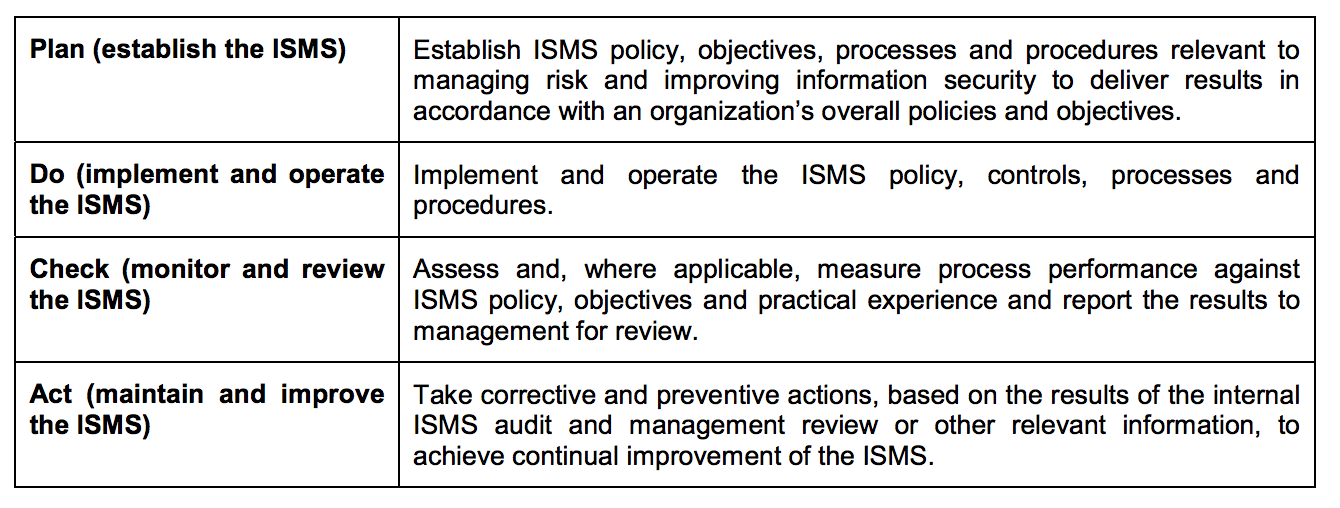
\includegraphics[width=\textwidth]{pictures/isms_concerns.png}
\caption{ISMS Stakeholder Concerns}
\label{fig:isms_stakeholder}
\end{figure}

Security requirements and objectives have to be defined in the earlier phases so they can be planned, implemented and carried out by the respective security architects/developers/security engineers. Here, the term user is not as clear since a variety of employees can be seen as such, e.g. any employee that accepts the established security policies. Since systems, as mentioned in Section \ref{sec:security}, are just as secure as the people using them, many employees can be viewed as ISMS users. They would be interested in implementing and operating the processes and procedures which have been defined in the previous phase.

Established security policies have to be also monitored and maintained. Security is never guaranteed and is a complex process \cite{vacca2012computer} - systems have to be constantly updated and possibly upgraded. 

The needs of the variety of security stakeholders have to be considered throughout the system processes and have to be registered in some way. Security requirements have been mentioned and, amongst others, will be described more thoroughly in the next section.

%\subsection{Enterprise Security}
%To define the term \textit{security concept} one has to look at the architecture of enterprises to understand the interconnectivity and interdependence between services, security being one of them. 
%
%\subsubsection{Enterprise Architecture}
%
%Information systems tend to be a very complex artifacts that combine different views and requirements from various stakeholders of different backgrounds \cite{alex}. 
%
%Software, IT platforms and IT related goals in general are covered in an \textit{Information System Architecture} (ISA). ISA does not take any business-driven influences into account and is therefore insufficient when describing the complex dependencies in corporations, especially when it comes to security as described in Subsection \ref{subsec:secarch}.   
%
%\textit{Enterprise Architecture Modeling} tries to overcome such possible difficulties and combines IT related concerns with business and organizational goals and shows possible interrelationships. It therefore provides an approach for an improved understanding of complex enterprise processes \cite{earch}. The Federal Deposit Insurance Corporation (FDIC) published the results of an audit of its own implementation of E-Government principles \cite{fdicaudit} and their division of information technology in Figure \ref{fig:fdic} depicts the interrelations very well. 
%
%\begin{figure}[H]
%\centering
%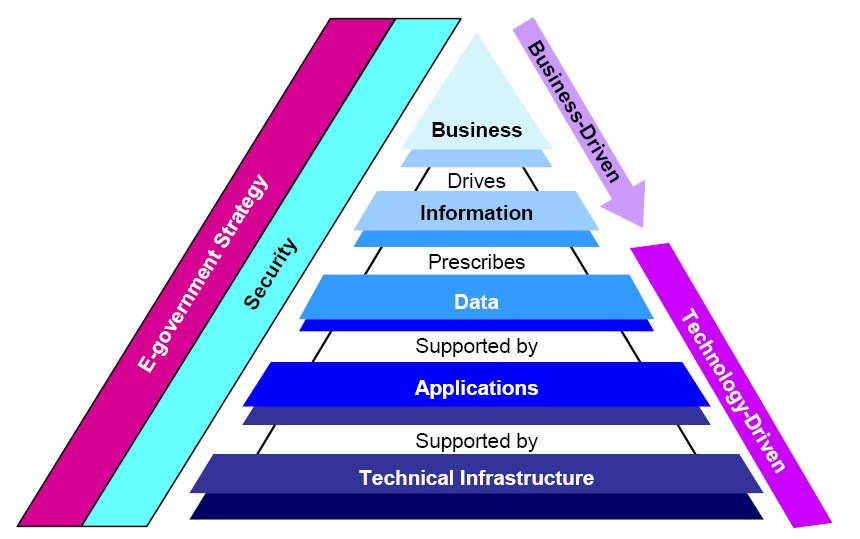
\includegraphics[width=0.75\textwidth]{pictures/fdic.jpg}
%\caption{Division of Information Technology by FDIC}
%\label{fig:fdic}
%\end{figure}
%
%\subsubsection{Security Architecture}
%\label{subsec:secarch}
%
%Information Security has often been merely an afterthought in corporations \cite{ansfederal} until a concept of a \textit{Security Architecture}, published in a whitepaper by The Gartner Group \cite{kreizman}, was introduced. According to \cite{kreizman} an \textit{Enterprise Information Security Architecture} (EISA) is an essential tool for improving security processes in corporations. EISA principles stand in a direct relationship with the EA principles and should be validated against them \cite{kreizman}. To highlight this relationship security considerations during phases of the \textit{The Open Group Architecture Framework Architecture Development Method} (TOGAF ADM), which is shown in Figure \ref{fig:togaf}, will be briefly described.
%
%\begin{figure}[H]
%\centering
%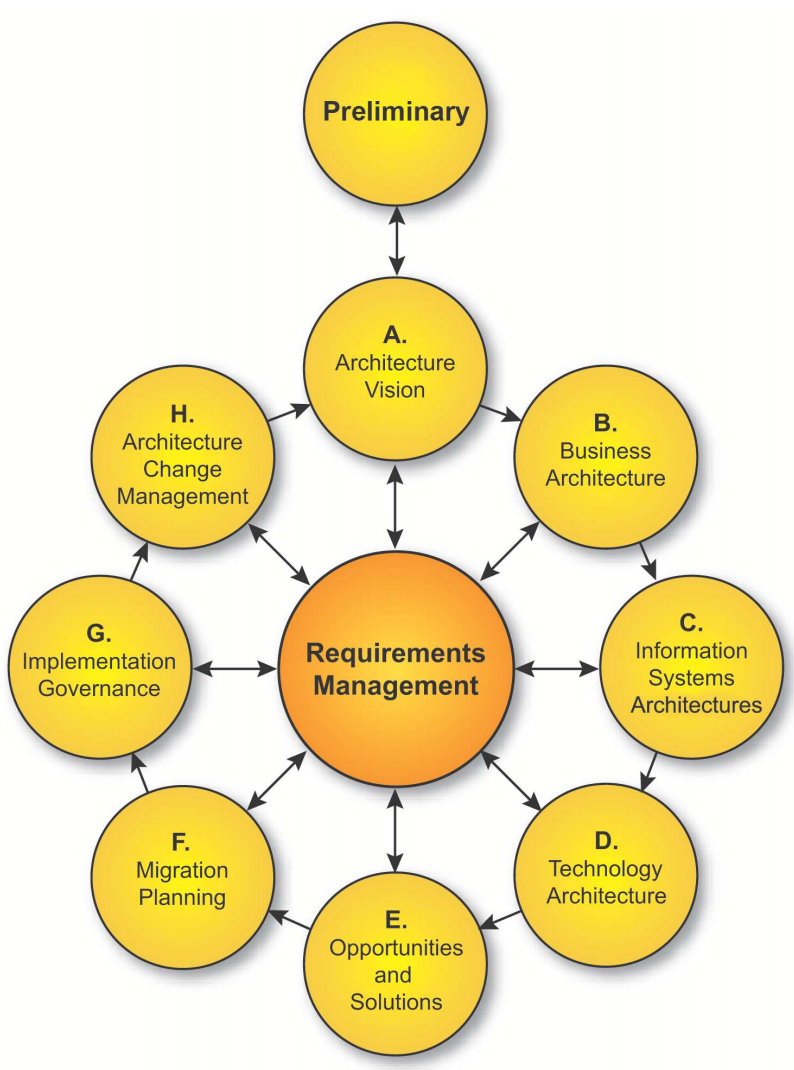
\includegraphics[width=0.6\textwidth]{pictures/togaf_overview.png}
%\caption{Overview of the phases of TOGAF}
%\label{fig:togaf}
%\end{figure}
%
%Security concerns can be found throughout the TOGAF phases which hints at the overall importance of security in corporations. TOGAF combines four architecture domains, the \textit{Business Architecture}, the \textit{Data Architecture}, the \textit{Application Architecture} and the \textit{Technology Architecture}. The following section will depict security considerations of two domains to show possible interrelations.
%
%During the \textit{Business Architecture} phase in the ADM actors and handlers of the system have to be identified. Costs and potential incoveniences because of security measures have to be assessed as well. In general one can say that the impacts of security/insecurity on the business/product are being highlighted. It is tried to put an emphasis on security as early as possible to prevent costly changes in later phases in the ADM.
%
%During the \textit{Information System Architecture} phase the classification levels of processed data have to be determined and documented. Direct dependencies to the \textit{Business Architecture} are also listed, e.g. the identification of information lifespan according to business goals and regulations. 
%
%Similar relations can be found for security considerations from various phases of the ADM. This once again shows the overall presence of security and the high level of complexity within an enterprise.

\subsubsection{Common Criteria}
The following section will present a way of modeling security concerns for an asset of interest.

Common Criteria proposes an evaluation by using a so called \textit{Security Target} (ST), a construct that encapsulates the \textit{Target of Evaluation} (TOE), threats to the TOE and countermeasures \cite{commoncriteria}. The goal of the evaluation is to show that the used countermeasures are sufficient to counter potential threats and thus implying that the TOE is sufficiently protected.

\begin{figure}[H]
\centering
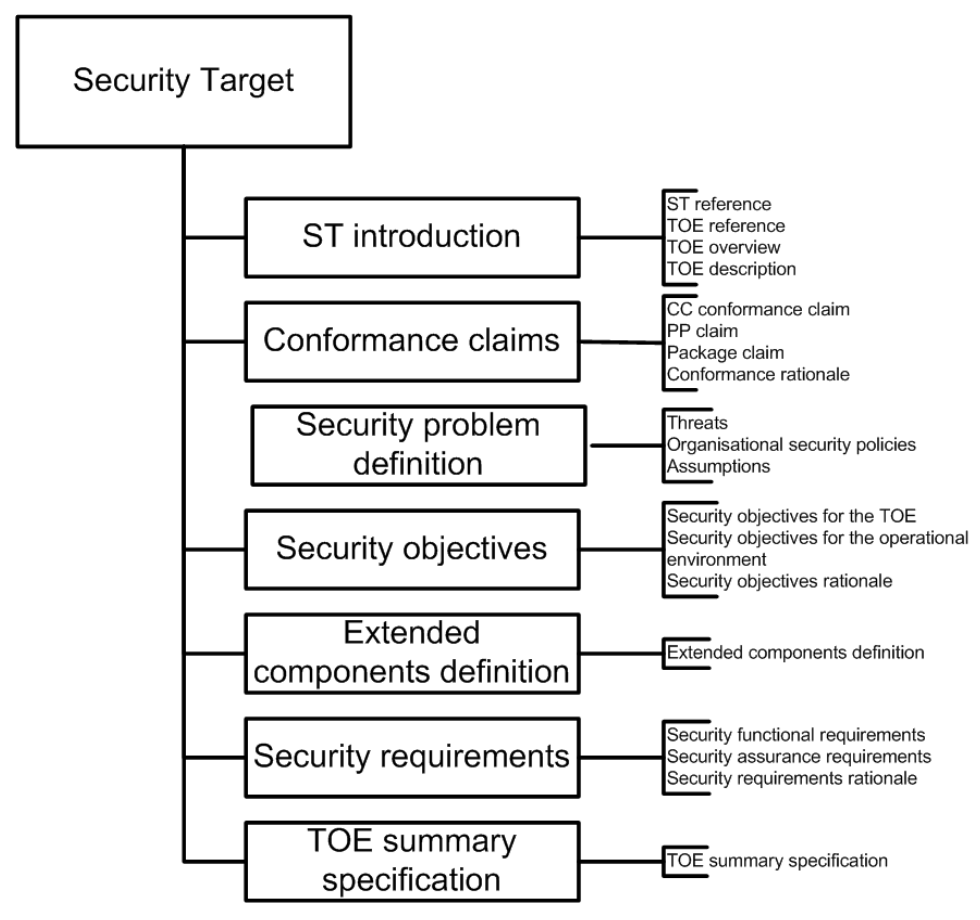
\includegraphics[width=0.85\textwidth]{pictures/sectarget.png}
\caption{Overview of the Security Target contents}
\label{fig:sectarget}
\end{figure}

A description of all the contents of a ST is unnecessary here and only the key security attributes of a ST that will be used to construct a \textit{Security Concept} (Subsection \ref{subsubsec:secconc}) are being introduced.

The \textit{Security Problem Definition} defines, as the name suggests, the security problem that is being addressed. Apart from containing guidelines and assumptions it contains \textit{Threats} which are \textit{\glqq[...] adverse actions performed by a threat agent on an asset\grqq} (\cite{iso27001}, p. 66).

A \textit{Security Objective} is an abstract solution to the previously defined security problem. There exists a possibility to divide the \textit{Security Objectives} into part wise solutions, one being the \textit{Security Objectives for the TOE} and the other being the \textit{Security Objectives for the Operational Environment}. Moreover does the ST contain traces showing which objectives address which threats, guidelines and assumptions and a set showing that all threats, guidelines and assumptions are addressed by the security objective.

\textit{Security Functional Requirements} (SFR) are a more detailed translation of the previously defined \textit{Security Objective}. Despite being more detailed, SFR have to be still independent from specific technical solutions. 

Lastly, STs contain a TOE summary specification where it is stated how the TOE meets all the SFRs and how exactly those requirements are met on a technical level.

\subsubsection{Security Concept}
\label{subsubsec:secconc}

The term \textit{Security Concept}, as it is defined here, is based on the constructs introduced in the previous chapters, namely \textit{Security Architecture} and \textit{Security Target}. An overview follows. 

\textit{Assets} are the to be secured objects of interest, i.e. TOE according to Common Criteria. \textit{Assets} can be either logical or physical and can be grouped to sets, if needed.

A \textit{Security Goal} (SG) is the equivalent to the \textit{Security Objective}. A valid SG must address an \textit{Asset} and a \textit{Security Goal Class} that defines the actual purpose of the SG. In general the set of \textit{Security Goal Classes} consists of \textit{Confidentiality}, \textit{Integrity} and \textit{Availability} but can also be expanded by further classes such as \textit{Authenticity}.

\textit{Threats} serve the same purpose as proposed by Common Criteria. They are adverse actions performed by an entity against an \textit{Asset}. 

This information is all brought together in \textit{Security Requirements} that are defined in natural language and show the interrelationships between elements. A \textit{Security Goal} has to be mentioned as well as an \textit{Asset} and a \textit{Threat} against which the object of interest should be protected.

Lastly, \textit{Controls} are the technical measures that counter or minimize the \textit{Threats}.     

The Table \ref{table:secconc} depicts the relationships between all the security attributes:

\begin{sidewaystable}
\begin{tabular}{|c|c|c|c|}
\hline
\textbf{Name} & \textbf{Contains} & \textbf{Description} & \textbf{Example} \\
\hline
\multirowcell{3}{Asset} & \multirowcell{3}{-} & \multirowcell{3}{Digital or physical object of \\ interest \\ that should be secured} & \multirowcell{3}{Sensible user data} \\
& & & \\
& & & \\
\hline
\multirow{2}{*}{Security Goal Class} & \multirow{2}{*}{-} & \multirowcell{2}{Defines the purpose \\ of the Security Goal} & \multirowcell{2}{Confidentiality of sensible \\ user  data} \\
& & & \\
\hline
\multirow{2}{*}{Security Goal} & \multirow{2}{*}{Security Goal Class, Asset} & \multirowcell{2}{Defines the security \\ objective} & \multirowcell{2}{ Confidentiality of sensible \\ user data shall be protected} \\
& & & \\
\hline
\multirow{2}{*}{Threat} & \multirow{2}{*}{Asset} & \multirowcell{2}{Adverse action against an \\ Asset} & \multirowcell{2}{Eavesdropping on sensible \\ user data} \\
& & & \\
\hline
\multirowcell{4}{Security Requirement} & \multirowcell{4}{Asset, Security Goal, Threat} & \multirowcell{4}{Security Objective \\ in natural language} & \multirowcell{4}{
The Confidentiality of \\ sensible user data shall \\ be protected against \\ eavesdropping} \\
& & & \\
& & & \\
& & & \\
\hline
\multirowcell{3}{Control} & \multirowcell{3}{Threat} & \multirowcell{3}{Measure to minimize \\ or mitigate the Threat} & \multirowcell{3}{Encryption of sensible user \\ data with AES-256 \\ to prevent eavesdropping} \\
& & & \\
& & & \\

\hline
\end{tabular}
\caption{Elements of a Security Concept}
\label{table:secconc}
\end{sidewaystable}

\subsection{Modeling}
\label{subsec:interpretation}
To ensure a viable solution one has to think of a representation of real life systems. \textit{Models} can be used to achieve this by depicting the key properties and processes of a certain system. According to Ed Seidewitz \cite{seidewitz} a model is a \textit{\glqq set of statements about some system under study\grqq} with the statements being either correct or incorrect.

A system modeled using the Unified Modeling Language (UML) serves as an example. In this case such statements could be made on the relationships between classes and would only be correct if they are consistent with the actual structure of the respective system under study (SUS), i.e. the described (modeled) relationships do indeed exist. 

In our case we would try to create a model that reflects the security attributes and their interrelationships in a SUS. This interpretation of a model is key because only then the model is given a meaning \cite{seidewitz}.

A definition of a model is not enough. A \textit{metamodel} has to be clearly defined to verify whether a model is conform or not, i.e. whether a security concept instance is conform to its security concept metamodel. The following figure shows the interrelationships.

\begin{figure}[H]
\centering
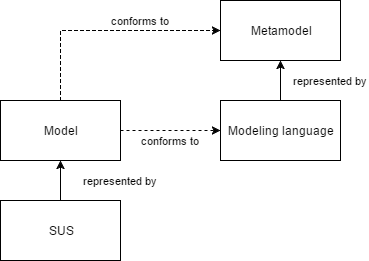
\includegraphics[width=0.65\textwidth]{pictures/metamodel.png}
\caption{Relationships between Model and Metamodel}
\label{fig:metamodel}
\end{figure}

A security concept of a SUS would be modeled in a modeling language, e.g. UML which is a representation of its own metamodel. At the same time the security concept would be conform to its metamodel. This conformity, be it the security concept or the modeling language, is needed for a model to be considered valid. 

\subsubsection{Model Transformation}
\label{subsubsec:modeltrans}
The Meta Object Facility (MOF) \cite{omg2013mof} is a standard metametamodel proposed by the Object Management Group (OMG) and captures the relationships between models in a three-layered architecture consisting of M1, M2 and M3. Models (M1) are representations of systems and are expressed in a modeling language M2, e.g. UML as mentioned in the previous section, which is conform to a so called metamodel. Metamodels themselves are also expressed in a metamodeling language which is conform to a metametamodel (M3). 

These architecture levels can be found in the \textit{model transformation pattern} by Jouault et al. \cite{modeltrans} which can be seen in Figure \ref{fig:metametamodel}. 

\begin{figure}[H]
\centering
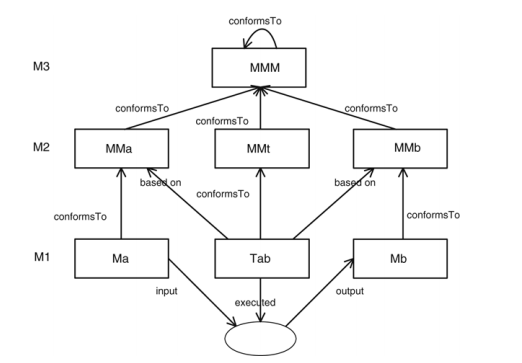
\includegraphics[width=\textwidth]{pictures/metametamodel.png}
\caption{Model transformation according to Jouault et al.}
\label{fig:metametamodel}
\end{figure}

Here a source model $Ma$ is being transformed into a target model $Mb$ using a transformation language. Both models and the transformation language are conform to their respective metamodel which is the traditional understanding of a model transformation but is unnecessarily complex for the security concept transformation.

Throughout the introduction and the background chapter the derivation of security attributes based on structural properties of a system of interest was mentioned. Given a model $M$ this derivation can be seen as alteration of $M$ and therefore as a \textit{model transformation}. The resulting model $M'$ is different to $M$, both however, are conform to the same metamodel $MM$. The transformation is being shown in Figure \ref{fig:transformation}.

\begin{figure}[H]
\centering
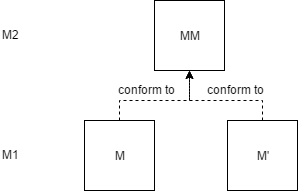
\includegraphics[width=0.55\textwidth]{pictures/transformation.png}
\caption{Model transformation}
\label{fig:transformation}
\end{figure}

The definition of a transformation $T$, or better a \textit{transformation rule set}, that alters a model $M$ is the main goal of this thesis.

Prior to the actual rule set definition one final concept has to be introduced. A user-selected \textit{Granularity level} serves as a second input in the model transformation.

\subsubsection{Granularity Levels}

Information systems are often complex because of the number of interconnections and interdependencies between components and therefore it might be difficult to assess potential impacts and risks of a system \cite{branagan}.

One logical goal would be to decrease the overall complexity to enable a better risk assessment. \textit{System abstraction} tries to achieve this by reducing the level of details \cite{branagan}. Branagan et al. differentiate between two possibilities, \textit{Whole-part decomposition} which decomposes a system into smaller subsystems and \textit{Distinct development perspectives} which focuses on certain parts of a system depending on the current development perspective. 

In this thesis the focus will be on the \textit{Whole-part decomposition} even though an adaption of development perspectives is certainly possible. The main difficulty would be the definition of such perspectives in the security context because they would be highly dependent on the respective security analyst. The perspectives would not be unambiguous.
  
Therefore the change of the level of detail, i.e. the granularity level, will be achieved by uniting or decomposing components of a system of interest. By decomposing a larger system into smaller subsystems one could focus on only specific security attributes and dismiss others.

A user will select a certain granularity level, i.e. a certain set of components, as an input to the transformation function $T$ as mentioned in \ref{subsubsec:modeltrans}. Together with the defined rule set a valid model $M'$ will be generated which to be considered valid has to be conform to its metamodel $MM$.

\section{Related Work}
\label{sec:related_work}

\section{Approach}
This section presents the approach addressing the previously mentioned goal of a model transformation based on the user-selected granularity level of a system of interest. Firstly, the security concept metamodel will be thoroughly described, each element of the metamodel will be put in the security context and advantages and disadvantages of such an interpretation will be highlighted.

The second part will deal with the actual transformation rules. Model transformations will be mathematically defined and the transformation rules for each element of the model will follow. Aside from the solution possible edge cases will be presented and evaluated.

\label{sec:approach}
\subsection{Security Concept}

The following metamodel is based on the security elements mentioned in Section \ref{subsubsec:secconc}. It shows the interconnections between elements and adds restrictions. This metamodel serves as a base enabling the creation of model instances capturing the relations between components/assets of a specific SUS. It also provides a security context and the option for the user to select a granularity level. 

\begin{figure}[H]
\centering
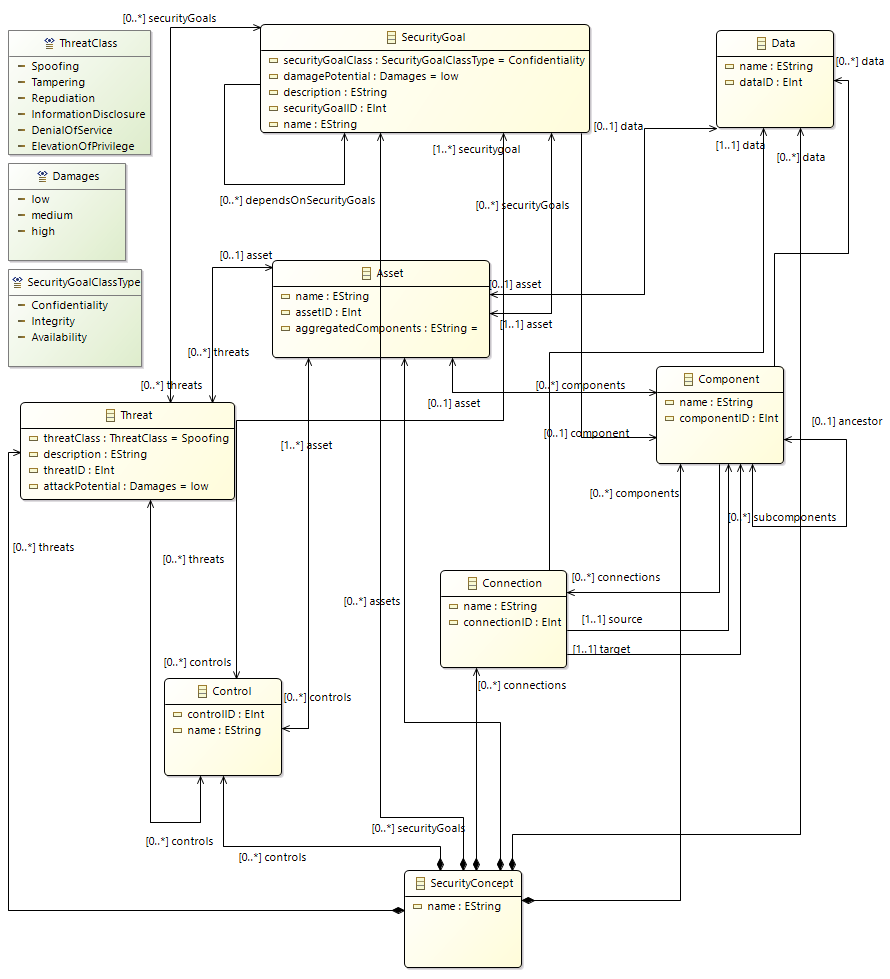
\includegraphics[width=\textwidth]{pictures/concept_metamodel.png}
\caption{Security Concept Metamodel}
\label{fig:concept_metamodel}
\end{figure}

In the figure above all the core elements \textit{Security Goal}, \textit{Asset}, \textit{Control} and \textit{Threat} are pictured. All of these elements are part of a \textit{SecurityConcept}, which in this model will be simply identified by a name. 

SGs have a \textit{Security Goal Class} attribute which describes the purpose of each SG. The \textit{Damage Potential} attribute indicates at the importance of a Goal, i.e. how important it is to secure a certain asset. The higher the damage potential the higher the impact if the security of an asset is breached. One key aspect of this metamodel is the dependency between SGs. A SG is dependent on another SG if both belong to the same asset and have the same security goal class. These dependencies, amongst others, have to be considered during potential transformation steps (Section \ref{subsec:secgoal}). 

Each SG belongs to exactly one asset whereas an asset itself can have unlimited SGs. In this thesis both physical and virtual components can be considered an asset. Both \textit{Data} and \textit{Component} can be assets according to the metamodel. 

There will be two different types of data. For once \textit{processed data}, i.e. data that is being processed or kept in storage by a specific component. On top of that \textit{transmitted data} will be considered separately since the transmission channel itself can be seen as an asset. The resulting interconnections are shown in the following figure:

\begin{figure}[H]
\centering
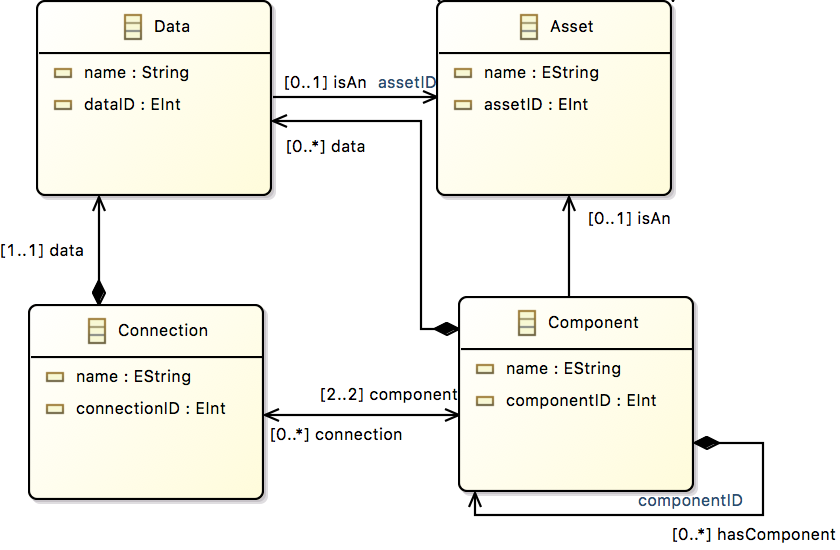
\includegraphics[width=0.65\textwidth]{pictures/two_data.png}
\caption{Two different interpretations of data}
\label{fig:data}
\end{figure} 

As already mentioned data can be viewed as being processed and transmitted. Therefore an element \textit{Connection} was added. A connection is the transmission channel between two components. It must have an associated data. The processed or stored data however can be directly associated with a component. In both cases data can be viewed as an asset. There is no possibility to assign a connection as an asset, the reason being that the transmission medium itself, i.e. the cable, wire, is rarely an object of interest but more so the data which is being transmitted.

Lastly the selection of \textit{Granularity Levels} by users should be enabled. Instead of having two different input models, one security concept model and one model depicting the system structure, one can reproduce the structural properties by adding a reference to the component element.      

\begin{figure}[H]
\centering
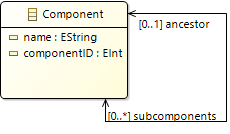
\includegraphics[width=0.45\textwidth]{pictures/component_structure.png}
\caption{Structural information}
\label{fig:data}
\end{figure} 

Having this extra reference one can create infinitely deep structural dependencies within the model. Therefore the actual transformation will only require one model instead of two separate ones.

\subsection{Metamodel elements and their security properties}
To put the different elements of the metamodel into a security context one has to clearly define the Security Goal Classes for possible assets. Interpretations of the classes are not unambiguous and it is necessary to discuss how security attributes propagate through different abstraction layers and what kind of impact interrelated components on different layers have on each other. 

\subsubsection{Components}

Before introducing the transformation rules one has to look at the different kinds of components that can be potentially found in a model instance. Even though the model element remains the same (\textit{Component}) a distinction which is made here is necessary because the interpretation of Security Goal Classes differs depending on the component type. 

\subsubsection*{Physical Component}

Physical components are components that can be accessed physically, e.g. computers, servers, switches etc. Since those can be accessed physically and therefore be manipulated physically one has to define the Security Goal Classes accordingly.

\begin{enumerate}
\item \textbf{Confidentiality} - Will be \textit{undefined} for physical components and will only hold for data stored/processed on those components
\item \textbf{Integrity} - Ensured when the component has not been altered by an adversary in any way; can be broken by an adversary having physical access
\item \textbf{Availability} - Ensured when the component is able to carry out its designated task; can be broken by an adversary having physical access
\end{enumerate}

\subsubsection*{Virtual Component}

Virtual components cannot be directly accessed physically. Examples would be virtual machines, virtual switches etc. The classes are similar to the physical counterpart except from the breach of the respective class.

\begin{enumerate}
\item \textbf{Confidentiality} - Will be \textit{undefined} for virtual components and will only hold for data stored/processed on those components
\item \textbf{Integrity} - Ensured when the component has not been altered by an adversary in any way; can be broken remotely by an adversary, i.e. without having physical access
\item \textbf{Availability} - Ensured when the component is able to carry out its designated task; can be broken remotely by an adversary, i.e. without having physical access
\end{enumerate}

\subsubsection{Data}

Similar to the component element the data element can be interpreted in different ways.
The distinctions between the different data types are very minor but noteworthy nonetheless. We consider three types of data, data which is being stored by a component, data which is being processed by a component and data which is being transmitted between components. The common terminology is \textit{Data at Rest}, \textit{Data in Motion} and \textit{Data in Use} \cite{kanagasingham2008data}. The used terms might be new, the distinction between different states of data however can be found in publications going as far back as 1982, e.g. by Dorothy E. Denning \cite{robling1982cryptography}.

\subsubsection*{Data at Rest}

Data at Rest applies to devices that hold data \cite{kanagasingham2008data}. An example would be a database containing sensitive information. The database being the \textit{Virtual Component} and the stored data being the \textit{Data at Rest}. One could also define the server with the database as a \textit{Physical Component}.

\begin{enumerate}
\item \textbf{Confidentiality} - Ensured when the data is protected from unauthorized disclosure at rest
\item \textbf{Integrity} - Ensured when the data is protected from unauthorized modification at rest
\item \textbf{Availability} - Ensured when the data is available to authorized parties when needed, i.e. authorized parties can access and use the data when needed
\end{enumerate}

\subsubsection*{Data in Use}

Data in Use applies to data that is being processed by a component, i.e. is being used by a service running on a component. An example would be data that is being processed by an API on a server. The API being the \textit{Virtual Component} and the server being the \textit{Physical Component}. The \textit{Data in Use} would be the processed information by the API backend.

\begin{enumerate}
\item \textbf{Confidentiality} - Ensured when the data is protected from unauthorized disclosure during processing
\item \textbf{Integrity} - Ensured when the data is protected from unauthorized modification during processing
\item \textbf{Availability} - Ensured when the data is available to authorized parties when needed, i.e. the data is being processed by the service/the respective service is running when needed
\end{enumerate}

\subsubsection*{Data in Motion}

Data in Motion applies to all data transmitted between components. We do not specify any protocols here to keep the definition as broad as possible.

\begin{enumerate}
\item \textbf{Confidentiality} - Ensured when the data is protected from unauthorized disclosure during transmission
\item \textbf{Integrity} - Ensured when the data is protected from unauthorized modification during transmission
\item \textbf{Availability} - Ensured when the data is available to authorized parties when needed, i.e. is not lost or intercepted during transmission 
\end{enumerate}

The different component/data types shown here should only show the different interpretations of the elements of the security concept metamodel. The interpretation of the element itself does not have an influence on the chosen metamodel element, i.e. the element for both physical and virtual components will still be \textit{Component}. The only difference can be found in data since transmitted data always belongs to a \textit{Connection}. For both processed and stored data however the metamodel element \textit{Data} will be used.

\subsubsection{Interpretation of Interconnections between Elements}

To describe model transformations in the security context one has to discuss how exactly the security attributes propagate through the respective abstraction layers. Here we will look into the dependencies between components and their security properties during transformations.

\subsubsection*{Sub-component}
\label{subsubsec:sub_comp}
A sub-component \textit{SC} will be defined as a component that directly belongs to a component \textit{C} which is in an abstraction layer above, i.e. encapsulates one or more sub-components. According to the previously defined metamodel such a relationship between components is being defined by the \textit{hasComponent} composition, i.e. a sub-component cannot exist without a component here. This also means that no new data types or structures are added when changing to higher granularity levels. Sub-components can only process data that has already been defined in the layers above. An example would be a database encapsulating a sub-component such as a secure key storage.   

\subsubsection*{Security Goals}

For security goals the interconnections between components and sub-components have to be interpreted in an unambiguous way. There is no clear definition on how SGs for components in higher abstraction layers propagate to the respective sub-components in the abstraction layers below. We therefore adopt the idea for security requirements which was proposed by Menzel et al. \cite{Menzel2008}. Here, the main focus will be on two characteristics, \textit{Independent} and \textit{Require} to capture interdependencies between SGs on different granularity levels. According to the metamodel each SG has the following attributes:

\begin{figure}[H]
\centering
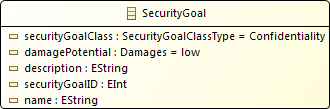
\includegraphics[width=0.65\textwidth]{pictures/securitygoal.png}
\caption{Attributes of a Security Goal}
\label{fig:security_goal}
\end{figure} 

The key attributes are \textit{securityGoalClass} and \textit{damagePotential}. Both are relevant when it comes to aggregation rules and dependencies amongst components. In this chapter the focus will be on the latter.

In case of a complete security concept definition interdependencies amongst components and security goals are clear, similar to Figure \ref{fig:subcomponent}. Out of simplicity security goals will be linked directly to components and not through assets.

\begin{figure}[H]
\centering
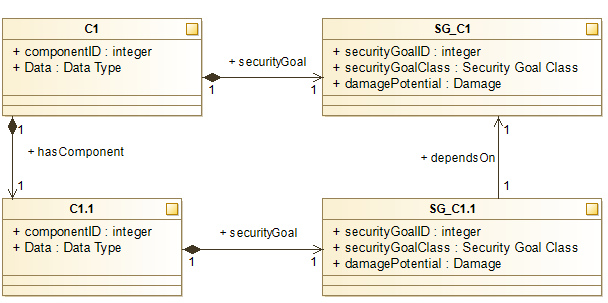
\includegraphics[scale=0.75]{pictures/rel_component.png}
\caption{Relationships between Security Goals}
\label{fig:subcomponent}
\end{figure} 

Figure \ref{fig:subcomponent} has shown the dependencies between components and their security attributes in case of a complete security concept definiton. In underspecified security concepts, such as shown in Figure \ref{fig:subcomponent_dilemma}, the dependencies are not as trivial. 

\begin{figure}[H]
\centering
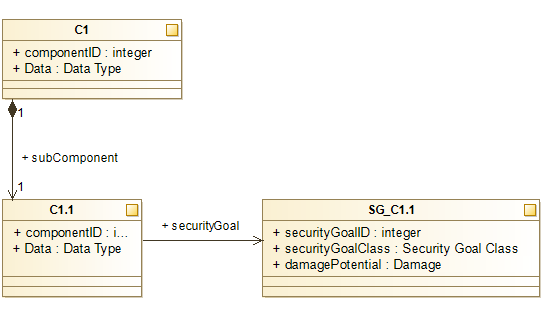
\includegraphics[width=0.75\textwidth]{pictures/sg_dilemma_no_goal.png}
\caption{Ambiguous propagation}
\label{fig:subcomponent_dilemma}
\end{figure} 

It is not obvious what kind of influence the sub-component has on its parental node, if at all. If the confidentiality of component $C_{1.1}$ is protected it is not clear how it will propagate to higher abstraction layers. Similar observations can be made for the aggregation from higher abstraction layers to lower ones. One has therefore to define when and how security attributes will propagate based on structural features of the SUS.

\begin{theorem}
A security goal $SG_{C_1}$ of a component $C_1$ has a direct influence on another component $C_2$ if and only if there is: 
\begin{enumerate}
\item a direct link between the two components, i.e. a hierarchical relationship between the two components AND
\item component $C_2$ processes/holds the data type that is being addressed by $SG_{C_1}$
\end{enumerate} 
\end{theorem}

This \textit{direct influence} is one of the more obvious dependencies amongst components. At first glance matching data types are needed to aggregate SGs through different abstraction layers but it is certainly possible that security concepts might be underspecified. Relying on this definition might therefore severely limit the transformation and thus, the resulting model.

An examplary model instance follows showing security attribute propagation with an underspecified security concept. Similarly to previous examples data/components will be directly linked with security goals without asset elements in between in the interest of greater clarity.

\begin{figure}[H]
\centering
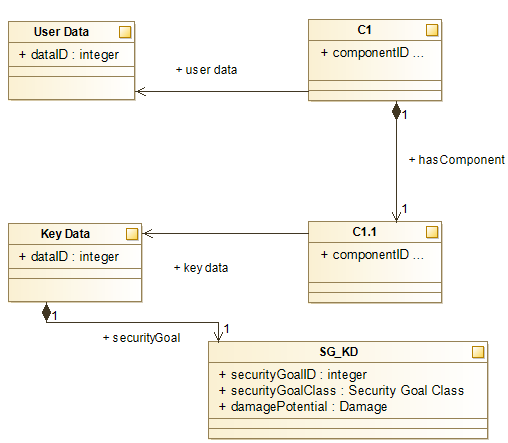
\includegraphics[width=0.75\textwidth]{pictures/sg_deduction.png}
\caption{Ambiguous propagation}
\label{fig:subcomponent_dilemma}
\end{figure} 

The corresponding security goal of the key data in natural text could be the following:

\begin{itemize}
\item[]\textbf{$SG_{KD}:$} The Confidentiality of sensible key data should be protected
\end{itemize}

Now we will look at component $C_{1.1}$ which has a link to key data. When looking through its SGs we will only find $SG_{KD}$ which should protect the \textit{Confidentiality} of said data. There is also a direct connection from $C_{1.1}$ to component $C_1$ which is in a granularity level above. 

According to the definition (Section \ref{subsubsec:sub_comp}) a sub-component can only process data that already exists in the abstraction layers above. Thus, a correct conclusion would be that if the confidentiality of key data is protected in $C_{1.1}$ it is also protected in the layer above even though there is no explicit link between $C_1$ and key data. This however, does \textit{NOT} mean that the overall confidentiality is being protected since $C_1$ may process other data, such 
as user data in the example.

Propagation from higher layers to lower ones is generally not possible without explicit links to data types. This will be discussed more thoroughly in Section \ref{subsec:sec_goals_rules}.

Similar conclusions can be made for the \textit{Integrity} of sub-components and its propagation to abstraction layers with higher or lower granularity levels with one slight difference. When looking at components at higher abstraction layers we can say that if the integrity of a component $C_1$ is being protected then all of its sub-components are being protected as well. 

For \textit{Availability} however, the situation differs. The connection between components (\textit{hasComponent}) has been defined as a composition. This means that the availability of a specific sub-component is pre-determined by the structural features of the SUS. If the availability of a component $C_1$ is protected it necessarily means that the availability of its sub-components is protected as well. To have the availability of a component protected however all of the sub-components have to be protected individually. The availability of a component is therefore the union of availabilities of its sub-components.

\subsubsection*{Threats}

Similar to SGs one can look into propagation rules for threats. Firstly we will look at the important attributes of a threat. The key attribute here will be \textit{attackPotential} which will be considered during the transformation steps in Section \ref{subsec:sec_goals_rules}.  
 
\begin{figure}[H]
\centering
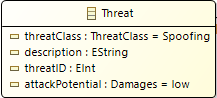
\includegraphics[scale=0.85]{pictures/threat.png}
\caption{Attributes of a Threat}
\label{fig:threat}
\end{figure} 

Here, the focus will be on the propagation of threats through granularity levels based on an underspecified security concept.

Every defined threat threatens at least one SG according to the metamodel (Figure \ref{fig:concept_metamodel}) and since every SG addresses one asset (component or data) we can use adapt the observations made in the previous section. 

\begin{figure}[H]
\centering
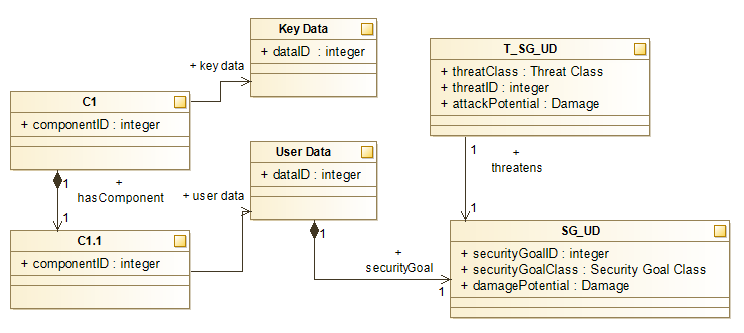
\includegraphics[scale=0.85]{pictures/threat_overview.png}
\caption{Underspecified Security Concept with a Threat}
\label{fig:threat_overview}
\end{figure} 

In Figure \ref{fig:threat_overview} a threat $T_{SG_{UD}}$ threatens $SG_{UD}$ which addresses the user data that is being used by sub-component $C_{1.1}$. The influence of $T_{KD}$ on higher abstraction layers is of interest since neither SGs nor threats are explicitly defined in the example.

\begin{itemize}
\item[]\textbf{$SG_{UD}:$} The Confidentiality of sensible user data should be protected
\item[]\textbf{$T_{SG_{UD}}:$} Eavesdropping on sensible user data
\end{itemize}

Similar to SGs, we can assume that $T_{SG_{UD}}$ propagates to the layer above based on the definition of sub-components. User data which is only explicitly addressed $SG_{UD}$ is also present at parental nodes. Thus, if the \textit{Confidentiality} of user data is being threatened by $T_{SG_{UD}}$, it is also being threatened when looking at $C1$.

For the propagation from abstraction layers depicting lower granularities ($C_1$) to layers with higher granularity ($C_{1.1}$) we have to take the data types into account. We will define a SG addressing key data and the corresponding threat.

\begin{itemize}
\item[]\textbf{$SG_{KD}:$} The Confidentiality of key data should be protected
\item[]\textbf{$T_{SG_{KD}}:$} Disclosure of key data
\end{itemize}

Now if the the confidentiality is being threatened by $T_{SG_{KD}}$ it is not clear how it will propagate to the layers below since $C_{1.1}$ is not addressing key data in any observable way. 

Threats that threaten SGs with \textit{Integrity} as their security goal classes behave in a very similar manner. Contrary to confidentiality, assumptions can be made when looking at propagation from higher abstraction layers to lower ones. When integrity of a component $C_n$ is being threatened the integrity of all respective sub-components $C_{n.1} ... C_{n.m}$ is being threatened as well. If the integritiy of a sub-component $C_{n.i}$ is being threatened it will also propagate to its parental node $C_n$ since a node can only be as secure as its sub-nodes.

Lastly, for \textit{Availability} the propagation is pre-determined by the structural features and the definition of sub-components. If the availability of a component $C_n$ is threatened it propagates to its sub-components $C_{n.1} ... C_{n.m}$. 

If the availability of one sub-component is being threatened it will also propagate to its parental nodes. This however does not mean that in case of an attack on the availability of $C_{n.i}$ the availability of $C_n$ will also be impaired. The availability of $C_n$ is a union of availabilities of its sub-components and one threat on a specific $C_{n.i}$ would alter said set.

We can therefore conclude that to ensure a SG of a component $C_n$ all its sub-components have to be protected as well. For threats however it is enough to threaten one sub-component to have an effect on its parental node.

\subsubsection*{Controls}

Controls try to mitigate threats and are directly linked to at least one threat at all times. The propagation of controls through abstraction layers will therefore be closely coupled with threats and SGs.

\begin{figure}[H]
\centering
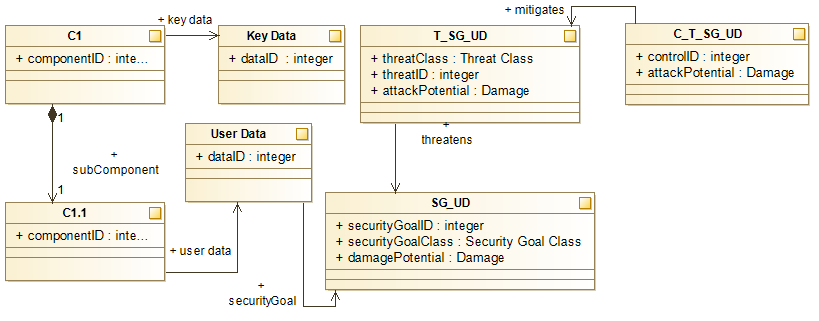
\includegraphics[width=\textwidth]{pictures/control_propagation.png}
\caption{Underspecified Security Concept with a Control}
\label{fig:control_propagation}
\end{figure} 

We have already discussed the propagation of SGs and threats in the previous chapters and thus, indirectly the propagation of controls. The example in Figure \ref{fig:control_propagation} shows a control that mitigates the threat $T_{SG_{UD}}$. In natural text the security attributes could be the following:

\begin{itemize}
\item[]\textbf{$SG_{KD}:$} The Confidentiality of sensible user data should be protected
\item[]\textbf{$T_{SG_{KD}}:$} Eavesdropping on sensible user data
\item[]\textbf{$C_{T_{SG_{KD}}}:$} Encryption of sensible user data with AES-256 to pevent eavesdropping
\end{itemize}

Similar to threats which propagate to the upper abstraction layers, controls will as well. The rules will be the same since the controls are very tightly coupled and cannot exist without threats.

For this example this would mean that when looking at the abstraction layer above and at $C_1$ we will consider the control $C_{T_{SG_{KD}}}$ as well the threat $T_{SG_{KD}}$ it is mitigating.

This section was only giving an overview on the conclusions for security attributes that can be made based on the structural features of an (underspecified) security concept definition. A more thorough definition will be discussed in the following section. 

\subsection{Model Transformation}

Let $SG_{CIA}$ be the set of security goals for a SUS. A security goal SG is defined as $SG(cl, asset, dmg)$ where $cl$ is the security goal class ($C$ for confidentiality, $I$ for Integrity and $A$ for availability), $asset$ being the element of interest which the SG was defined for and $dmg$ is the damage potential in case of a security breach ($H$ = high, $M$ = medium and $L$ = low).

\subsection{Transformation Rule Set for Security Goals}
\label{subsec:sec_goals_rules}
\subsubsection{Aggregation Rules}
\subsection{Transformation Rule Set for Threats}
\label{subsec:threat_rules}
\subsubsection{Aggregation Rules}
\subsection{Transformation Rule Set for Controls}
\subsubsection{Aggregation Rules}

\section{Implementation}
\subsection{Technology}
\subsection{Validity \& Verification}
\subsection{Runtime \& Complexity}

\section{Summary}
\section{Outlook}
\label{subsec:secgoal}